\chapter{Grundlagen}

\section{Die 4. industrielle Revolution}

Der Grundgedanke von Industrie 4.0 ist die flächendeckende Vernetzung von Informations- und Kommunikationstechnik zu einem Internet der Dinge, Dienste und Daten. (Spath, 2014 - TODO ref.)

\subsection{Historie}
TODO - Industrie 3.0 -> Industrie 4.0 - Kommunikation über Unternehmensgrenzen

TODO - Beschreibung der unternehmensinternen Kommunikation der Systeme mit Hinblick auf die Automatisierung der Industrie in der dritten Revolution.

\begin{figure}[h]
  \centering
  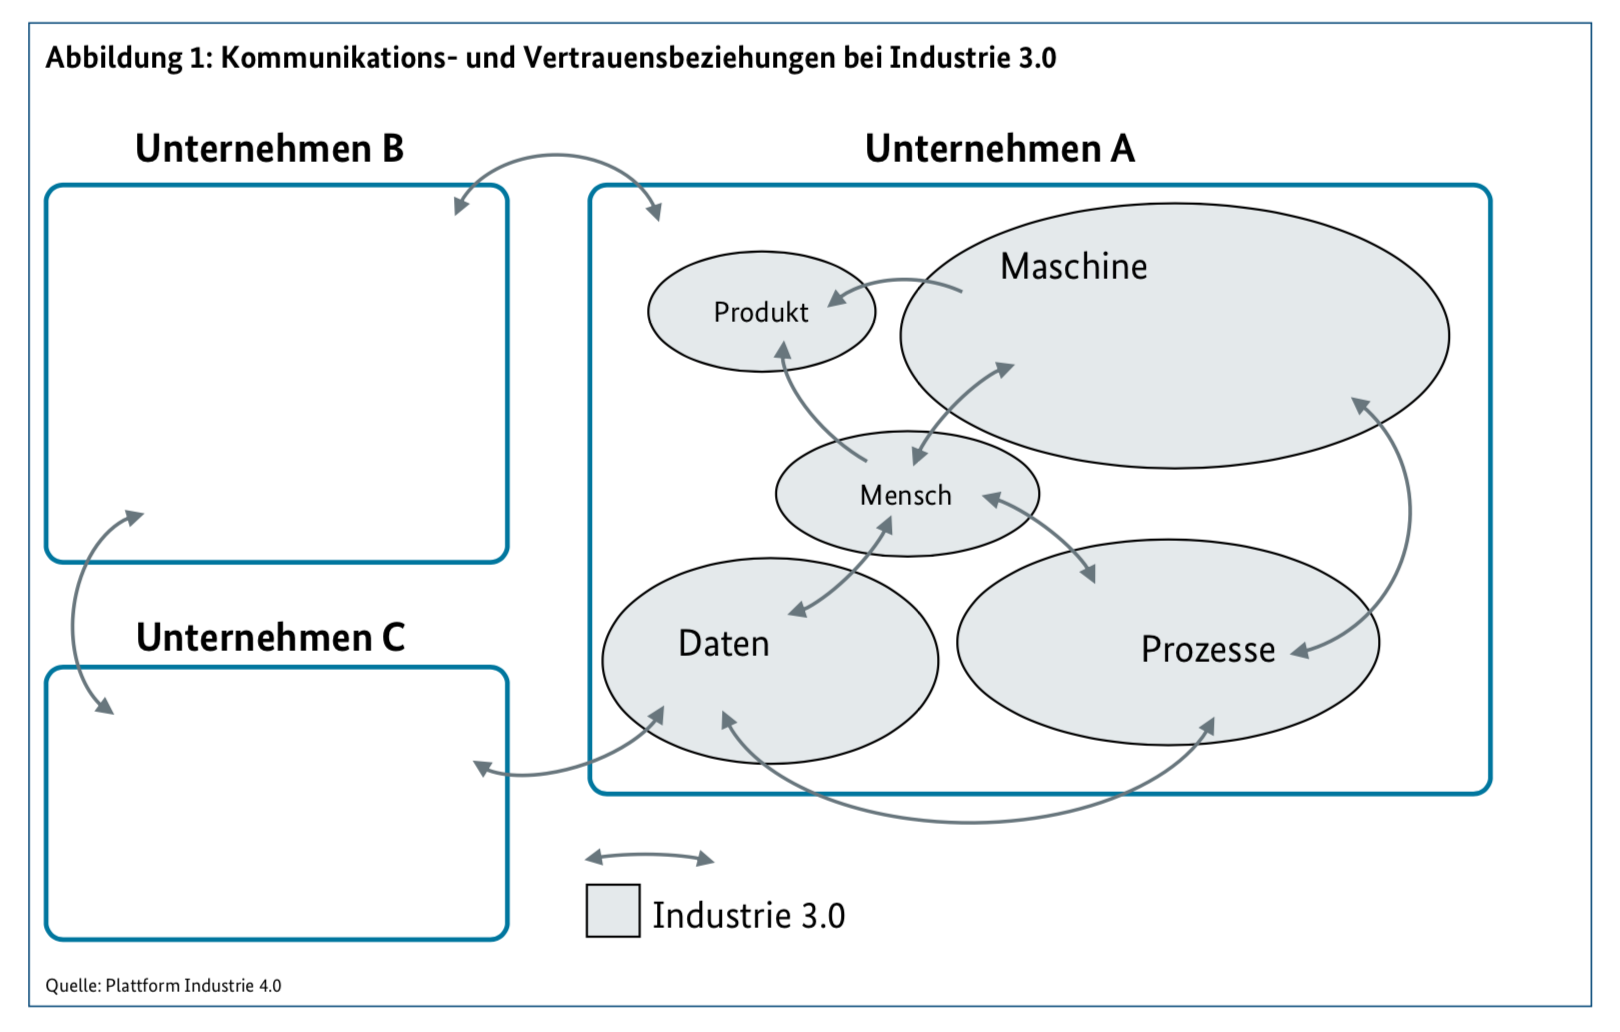
\includegraphics[width=15cm]{kommunikationsbeziehungen-i30}
  \caption{Kommunikationsbeziehungen in einer Industrie 3.0 Umgebung - TODO ref. sichere unternehmensübergreifende Kommunikation}
  \label{Kap2:Industrie3.0-Kommunikation}
\end{figure}

\clearpage

TODO - Beschreibung der unternehmensübergreifenden Kommunikation in Industrie 4.0 Umgebungen.

\begin{figure}[h]
  \centering
  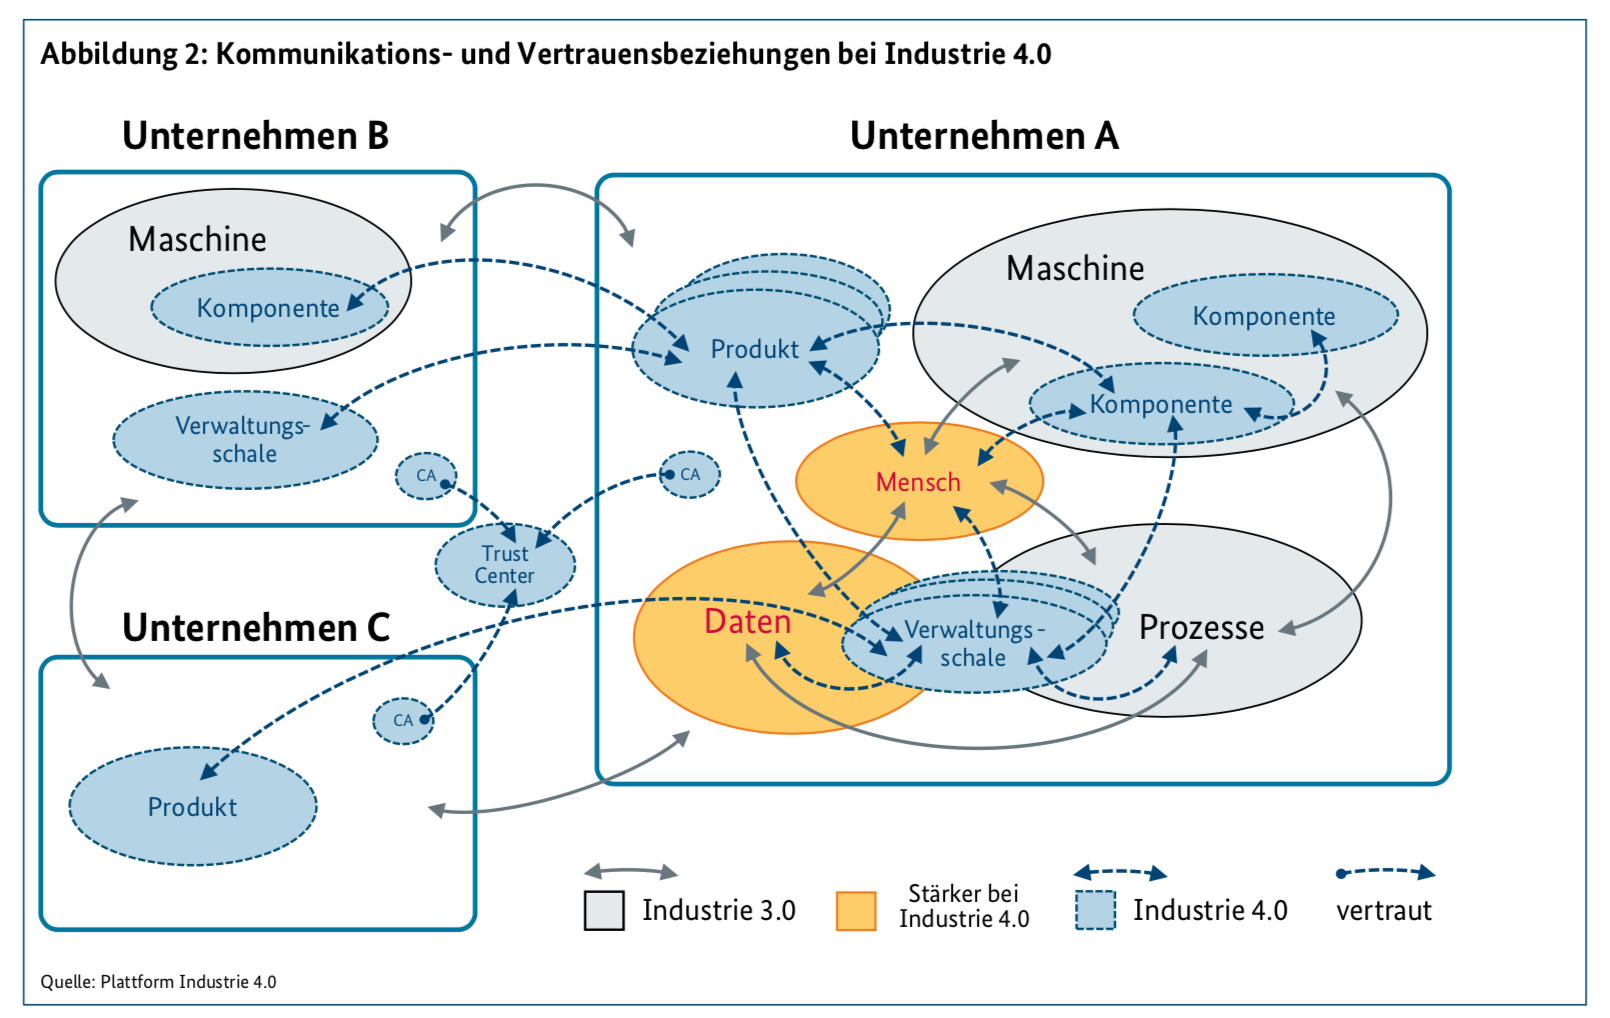
\includegraphics[width=15cm]{kommunikationsbeziehungen-i40}
  \caption{Kommunikationsbeziehungen in einer Industrie 4.0 Umgebung - TODO ref. sichere Unternehmensübergreifende Kommunikation}
  \label{Kap2:Industrie4.0-Kommunikation}
\end{figure}

\clearpage

\subsection{Aktueller Stand der Technik}
Die Entwicklung der Industrie zu ihrer vierten Revolution ist ein stetiger, nicht abgeschlossener Prozess. Aktuell werden die ersten Smart Factories der Industrie errichtet und erste smarte Einkaufsmöglichkeiten, wie Amazon Go, für den Endverbraucher geschaffen. Diese Fabriken und Filialen stellen die ersten ihrer Art dar und dienen als Prototypen. Das Ziel des Wandels in der Strukturierung und Organisation der Produktion in Unternehmen ist eine immer weitere Automatisierung der Prozessabwicklung bis hin zu autonom arbeitenden Fabriken.

\subsection{\ac{RAMI4.0}}
TODO - notwendig? Schichtenmodell, Darstellung eines Assets. nur kurze Beschreibung? wenig Bezug zur Netzwerkkommunikation. Smart Sensors, Kommunikationsfähigkeit eines Assets (aktiv,passiv)

\subsection{Automatisierungspyramide}
Die Automatisierungspyramide stellt die beteiligten Systeme und Softwarekomponenten eines automatisierten Prozesses systematisch dar. Diese beginnen, ausgehend vom Kundenauftrag und der betriebswirtschaftlichen Planung der Produktion auf der Unternehmensebene im \ac{ERP} System. Die Ergebnisse der Planung werden an das \ac{MES} übergeben, welches die verschiedenen Fertigungs- oder Logistikaufträge generiert. Die Aufträge werden anschließend auf der Prozessleit- (\ac{SCADA}), Steuerungs- (\ac{SPS}) und Feldebene (Ein-/Ausgangssignale) bearbeitet.

\begin{figure}[h]
  \centering
  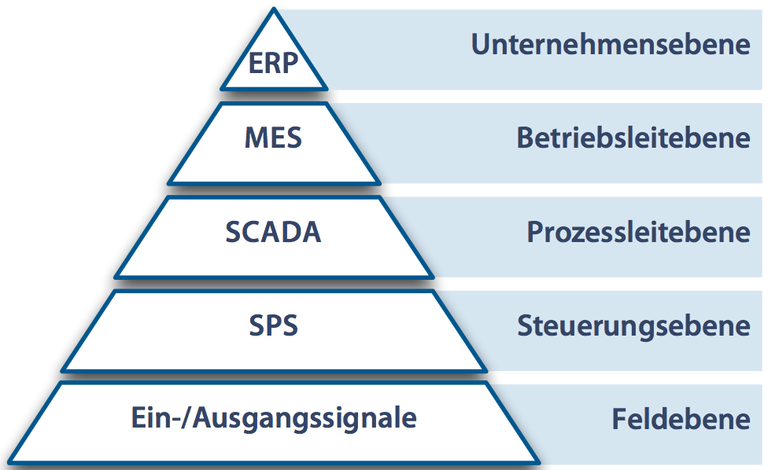
\includegraphics[width=10cm]{automatisierungspyramide}
  \caption{Automatisierungspyramide - TODO ref. Langmann,2004}
  \label{Kap2:Automatisierungspyramide}
\end{figure}

\clearpage

Während die oberen Schichten der Pyramide (\ac{ERP} und \ac{MES}) durch Standardkomponenten bzw. -software der IT realisiert werden, zählen die unteren Schichten (Prozessleit- bis Feldebene) zur Automatisierung, welche die Steuerung und Kontrolle der technischen Anlagen übernimmt. Diese werden auch als Shop-Floor-Ebene bezeichnet. Sie sind durch spezielle Hard- und Softwarelösungen umgesetzt. Die Kommunikation dieser Systeme ist u. a. für spezielle Anwendungsfälle wie harte Echtzeitreaktionszeiten mit Verzögerungen <1ms ausgelegt. Die Integration von Sicherheitsmaßnahmen bei der Kommunikation dieser Systeme stellt oft eine große Herausforderung dar.

\section{Grundprinzipien der sicheren Kommunikation}
\subsection{Vertraulichkeit/Zugriffsschutz}
\subsection{(Daten-)Integrität/Änderungsschutz}
\subsection{Authentizität/Fälschungsschutz}
\subsection{Verbindlichkeit/Nichtabstreitbarkeit}
\subsection{Anonymität}

TODO - Industrie 4.0 beinhaltet durch die Unternehmensübergreifende Kommunikation außerdem den rechtlichen Rahmen, welcher bei Nichteinhaltung von Verträgen bzgl. Verfügbarkeit, Integrität und Vertraulichkeit gelten kann.

\section{sichere Kommunikation in Industrie 4.0}
Im Gegensatz zur I3.0, in welcher Daten auf lokaler Ebene oder zwischen einzelnen internen Unternehmensebenen ausgetauscht wurden, stellt in der I4.0 der Austausch von Daten und Informationen über Unternehmensgrenzen hinweg eine wesentliche Herausforderung dar. Dabei findet die Kommunikation nicht mehr über ein Enterprise-Resource-Planning-System (ERP) statt, sondern auch direkt von einer darunterliegenden Ebene, wie z. B. einer Maschine mit ihrem Lieferanten. Durch diese enge Vernetzung können sowohl Menschen, als auch Maschinen die Kommunikationspartner sein.

\subsection{Anforderungen}
\subsection{Komponenten einer I4.0 Architektur}
\subsubsection{Assets}
\subsubsection{Smarte Sensoren}
\subsubsection{TODO}

\subsection{Kommunikationsstrukturen}
\subsubsection{End2End}
\subsubsection{Gateways}
\subsubsection{Publish-Subscribe}
\subsubsection{Kommunikation mit Netzwerk als Partner}